\chapter{Grundlagen} 
\label{cha:Grundlagen}


\section{Java Virtual Machine} 
\label{sec:Java Virtual Machine}
% java einleitung
Gemessen am Interesse der Anwender und an seiner Verbreitung ist Java die erfolgreichste Programmiersprache der letzten Jahre. Der Erfolgt kam mit der Objektorientierung sowie der Plattformunabhängigkeit. Diese Fähigkeiten brachten eine große und fähige Kommune zusammen, die sowohl aus der Wirtschaft als auch aus der Forschungsbereich besteht. Dementsprechend ist Java im Laufe der Zeit durch Designmustern, Architekturkonzepten, Paradigmen und aktuellen Sicherheit- sowie Industriestandrats erweitert worden. Da Renew mit Hilfe der Java Plattform umgesetzt wurde, kann sie sie sich alle gegebenen Vorteile zunutze machen. 
Einer der wichtigen Bausteine von Java ist die virtuelle Maschine, die das Suchen, Laden und Ausführen einer Codebasis auf allen gängigen Betriebssystemen erlaubt. Dementsprechend spielt das Laden von Klassen aus Örtlich unabhängigen Plugins ein große Rolle für die entstandene Architektur. Die Plugins müssen gefunden, geladen und kommunikationsfähig eingerichtet werden, sodass sie sich gegenseitig nutzen und beeinflussen können. \newline 
In diesem Kapitel werden grundlegende Konzepte des \textit{ Classpath's, Classloader's und Reflaction} erläutert mit Hilfe dessen die Renew Plugin-Architektur umgesetzt wurde.

\subsection{Classpath}
\label{sub:Classpath}
% classpath einleitung
Jede Java-Anwendung wird zuerst in einer für menschlich verständlichen Sprache geschrieben und anschließend in ByteCode übersetzt. In Folge dessen ist der Code bereit zur Ausführung und muss an die virtuelle Maschine weiter gereicht werden.\newline
Um die compilierten Klassen zu laden, wird von der JVM(Java Virtual Machine) Ortsangaben mit entsprechenden Code erwartet. Die Ortsangaben nennt man \textit{Classapth} oder Klassenpfad. Dieser beschreibt eine Liste von Orten an denen sich die zur Ausführung benötigten Klassen befinden, wie zum Beispiel das lokalen Dateisystem, das Netzwerk oder sogar die Datenbank. Nachdem der Klassenpfad für die entsprechenden Classloader gesetzt ist, kann das \textit{Classlaoder System} die gewünschten Klassen erfassen und in die virtuelle Maschine laden.

% simple classloader image 
\begin{figure}[h]
  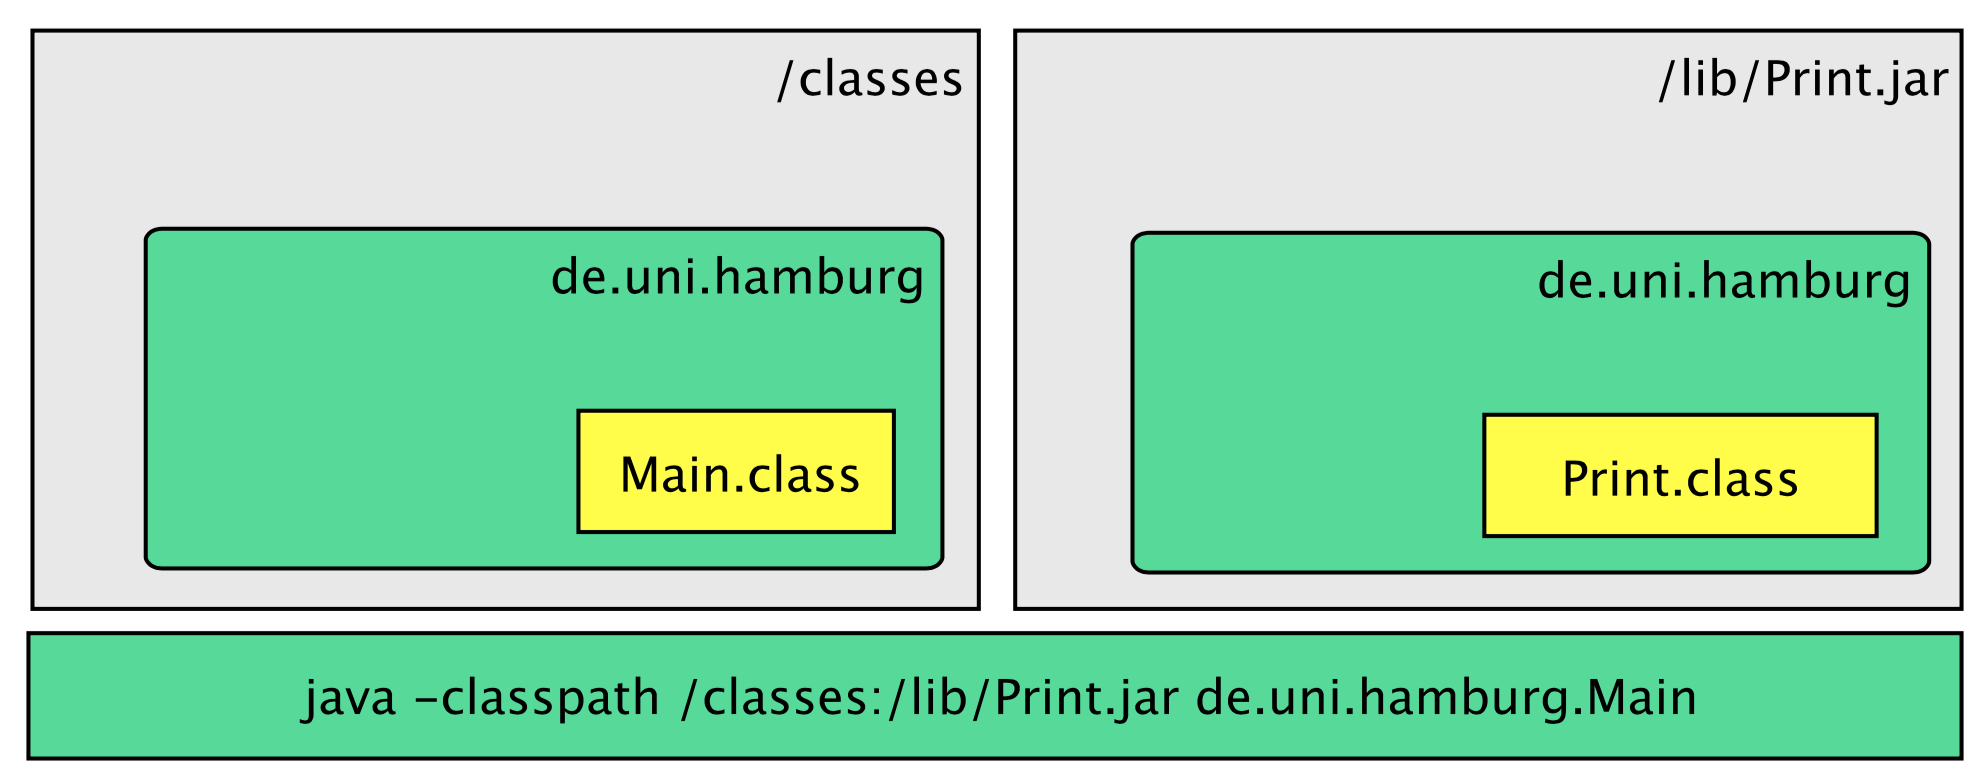
\includegraphics[width=\textwidth]{material/images/Classpath.png}
  \caption{Java Classpath}
  \label{fig:Classpath-Simple}
\end{figure}

% simple classloading 
 In Beispiel [\ref{fig:Classpath-Simple}] besteht der Klassenpfad aus einem Ordner sowie einem JAR-Archive, die für die Ausführung nötige Klassen beinhalten. Da beide Orte eine Dateistruktur beinhalten unterliegen sie einer Einschränkung, beide müssen die Paketstruktur der Java Klassen widerspiegeln damit der \textit{Applikation Classloader} diese durchsuchen kann. Abschließend braucht Java einen Startpunkt, mit dem die Applikation ihre Ausführung beginnt. Jedes mal wenn eine Klasse instantiiert werden muss, wird der \textit{Classpath} von Links nach Rechts nach dem benötigten Typ durchsucht und instantiiert. Somit hat der Klassenpfad eine interne Ordnung und eine Abarbeitungsreihenfolge.
\begin{figure}[h]
  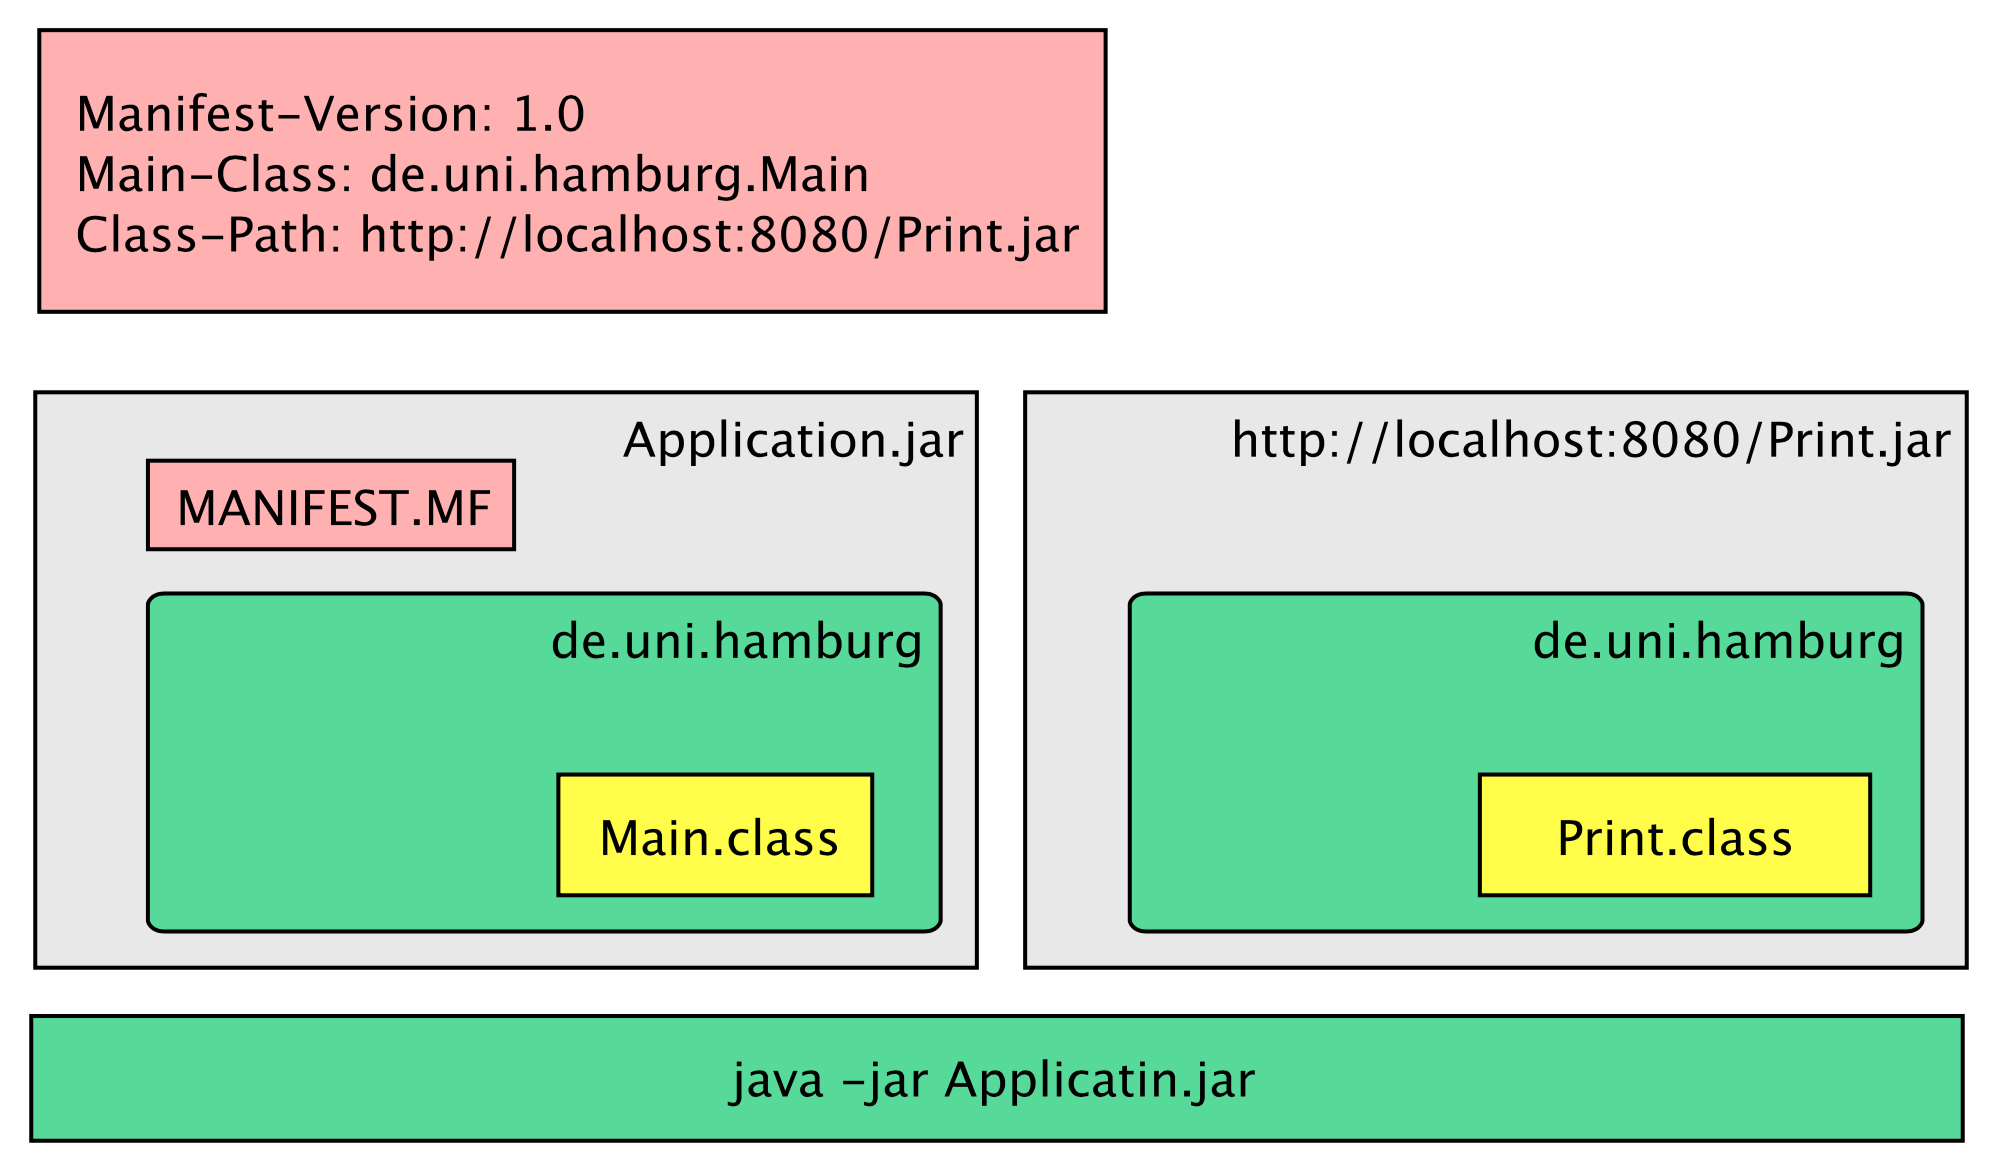
\includegraphics[width=\textwidth]{material/images/Classpath-Manifest.png}
  \caption{Jar Classpath}
  \label{fig:Classpath-Advanced}
\end{figure}

% jar classloading with manifest 
Im Beispiel [\ref{fig:Classpath-Simple}] wurde explizit ein Applikationsklassenpfad gesetzt, der für die Ausführung benötigten Klassen zuständig ist. Für den Ablauf großer Applikationen mit viele Abhängigkeiten kann dieser ausgedehnt und chaotisch werden. Von daher bietet Java eine Archivstruktur, die einen standardisierten Aufbau sowie zusätzliche Meta-Information über den Container in sich trägt. Mit Hilfe der Strukturrichtlinie befindet sich der komplette Inhalt eines Archivs auf dem Applikationsklassenpfad und kann zusätzlich in der \textit{manifest.mf} Datei erweitert werden. Die \textit{manifest.mf} spielt eine große rolle in der Entwicklung von Java Applikation, diese kann den Namen, die Version, den Entwickler und die Sicherheitsattribute tragen, die während der Laufzeit ausgewertet werden können. Zum Beispiel wird in [\ref{fig:Classpath-Advanced}] der Klassenpfad durch ein Archive aus dem web erweitert und für die Ausführung genutzt. Des weiteren hält die \textit{manifest.mf} einen Einstiegspunkt für die Ausführung, der auf eine Klasse mit der \textit{main} Methode verweist. Somit kann die Applikation in einer kurzen und einfachen Form gestartet werden, da der Ausführungskontext durch die Struktur und die mitgelieferten Meta-Information komplett ist.

\subsection{Classloader}
\label{ssub:classloader}
In den vorherigen Beispielen[\ref{fig:Classpath-Simple}, \ref{fig:Classpath-Advanced}] wurde die Bedeutung und die Rolle des Klassenpfads für die Applikation beschrieben, dennoch muss dieser zuerst verarbeitet werden. Diese Aufgabe wird von dem \textit{Classloader} übernommen, der eine zentrale Rolle in jeder Applikation spielt. Zumal er nach benötigten Java Klassen für die Instantiierung der entsprechenden Typen sucht. Da es eine wichtige Aufgabe ist, wird die Verantwortung für das Laden der Klassen über eine Menge von \textit{Classloader} aus dem \textit{Classloader System} aufgeteilt. 

\subsubsection{Classloader System}
Das \textit{Classloader System} besteht aus drei integrierte \textit{Classloader}, von denen jeder einen anderen Gültigkeitsbereich für das Laden der Klassen besitzt. Beim Abstieg der Hierarchie wird der Umfang der verfügbaren Quellen breiter und weniger vertrauenswürdig. 
%Die Idee hinter dem Separieren der Aufenthaltsorte ist, dass den Quellen unterschiedliche Vertrauensebenen zugewiesen werden können.
\begin{figure}[h!]
  \centering
  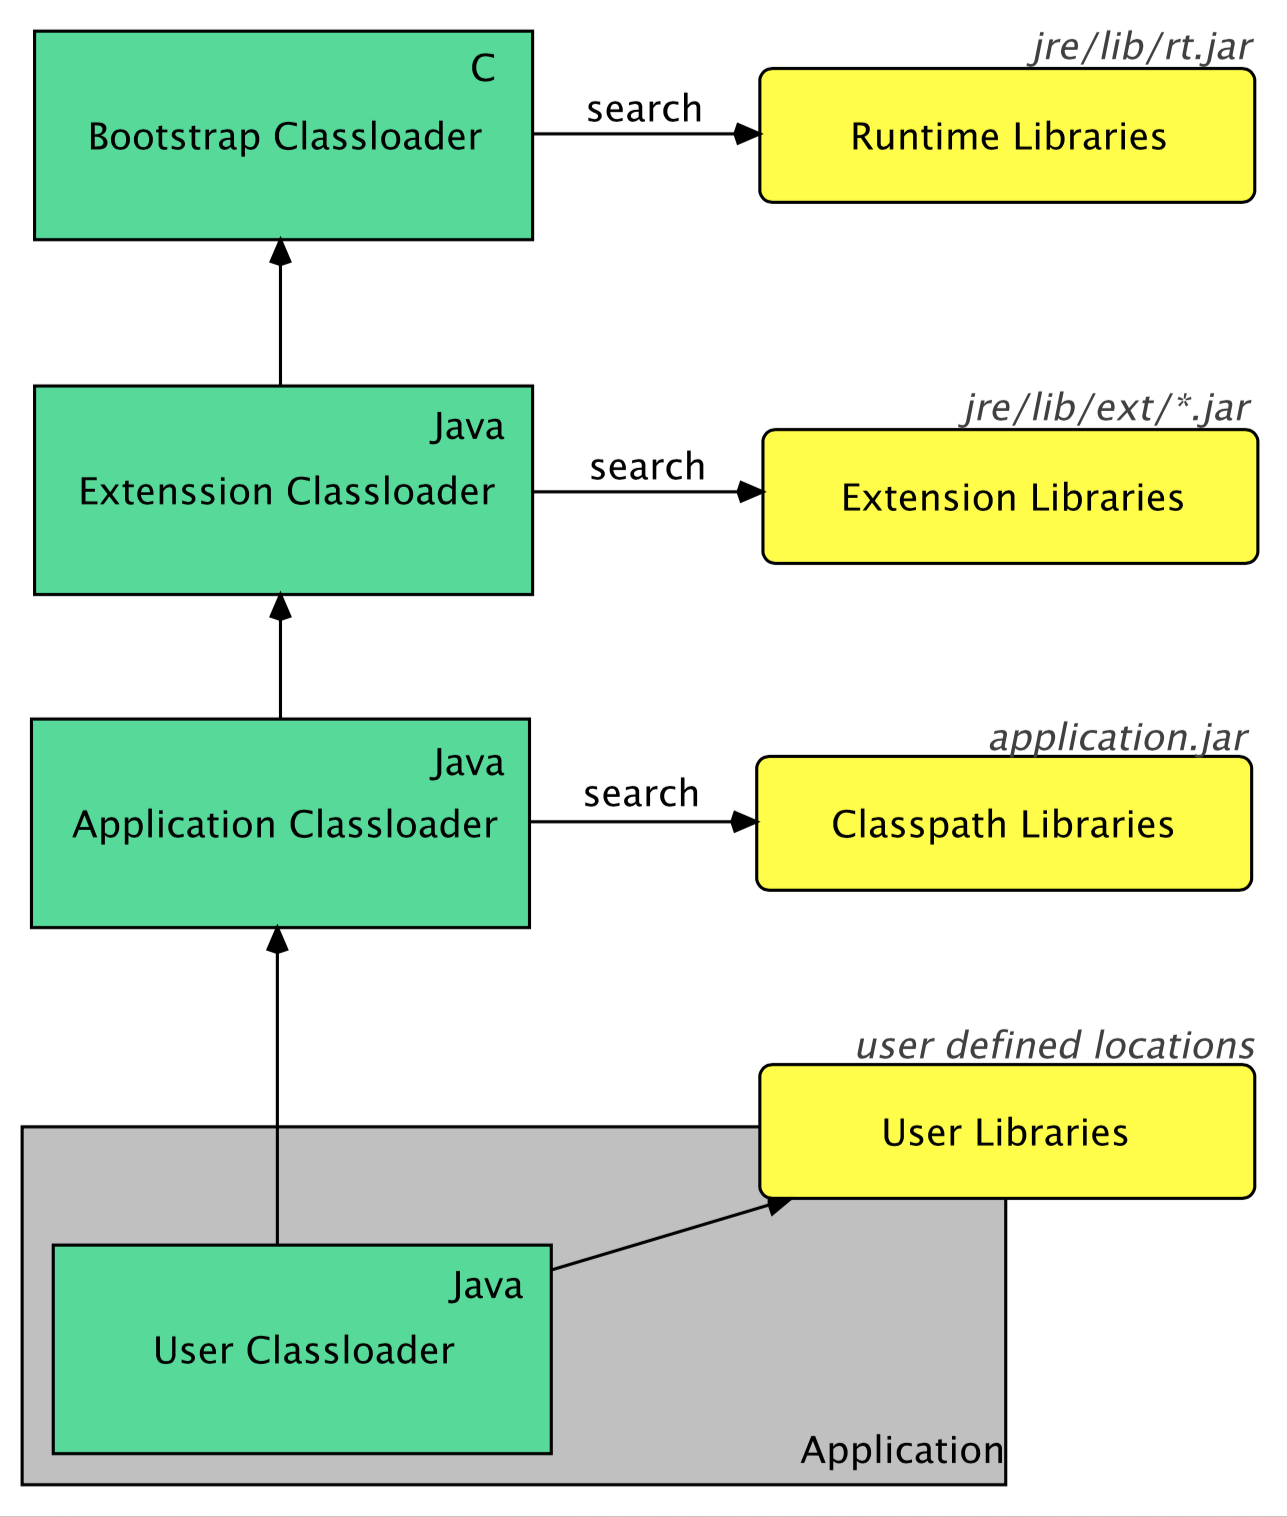
\includegraphics[width=0.7\textwidth]{material/images/Classloader.png}
  \caption{Classloader System}
  \label{fig:Classloader}
\end{figure}
\newline
Oben in der Hierarchie befindet sich der \textit{Bootstrap-Classloader}. Dieser \textit{Classloader} ist verantwortlich für das Laden der grundlegenden Java Klassenbibliothek, wie die zum Beispiel Java-Core-API aus der \textit{rt.jar}. Diese Klassen sind am vertrauenswürdigsten und werden zum Starten der virtuellen Maschine verwendet. Der \textit{Classloader} für Erweiterungen kann Klassen laden, die Standarderweiterungspakete im Erweiterungsverzeichnis \textit{lib/ext} sich befinden. Diese können Java-UI wie kryptografische Erweiterungen beinhalten. Der darunter liegende \textit{Applikation Classloader} ist zuständig für unseren Code und lädt Klassen aus dem allgemeinen Klassenpfad einschließlich der zu startenden Anwendung. Zuletzt können Benutzerdefinierte \textit{Classloader} erstellt werden, die sich auf der unteren Ebene der Classloader-Hierarchie befinden und auf Drittanbieter Bibliotheken zugreifen können. Demzufolge sind diese Quellen nicht sicher genug um ihnen große Priorität zuzuweisen, wie zum Beispiel den geladenen Klassen des \textit{Bootstrap-Classloader}. 
\bigbreak
Dieses System verhindert, dass Code aus weniger sicheren Quellen vertrauenswürdige Core-API-Klassen ersetzt, indem der selbe Name als Teil der Core-API angenommen wird. Daraus folgt ein Delegierungsmodell, welcher eindeutige Klassen garantiert, da die Klassensuche von Oben nach Unten der Classloader-Hierarchie abgearbeitet wird. [\ref{fig:Classloader}] 
  
\subsubsection{Delegierungsmodell}
Das \textit{Classloader System} delegiert jede Anfrage zum Laden einer bestimmten Klasse zuerst an seinen übergeordneten \textit{Classloader}, bevor der angeforderte \textit{Classloader} versucht die Klasse selbst zu laden. 
Jeder \textit{Classloader} hält somit einen Verweis auf einen übergeordneten \textit{Classloader} und ist Teil eines \textit{Classloader} Baums mit dem \textit{Bootstrap-Classloader} an der Wurzel. Wenn eine Instanz einer bestimmten Klasse benötigt wird, prüft der \textit{Classloader}, der die Anfrage bearbeitet, normalerweise mit seinem übergeordneten \textit{Classloader} vorab. Der übergeordnete \textit{Classloader} durchläuft wiederum den gleichen Prozess bis die Delegierungskette den \textit{Bootstrap-Classloader} erreicht. Sobald der \textit{Bootstrap-Classloader} erreicht wurde, beginnt die tatsächliche Suche nach der gewünschten Klasse.
\begin{figure}[h]
  \centering
  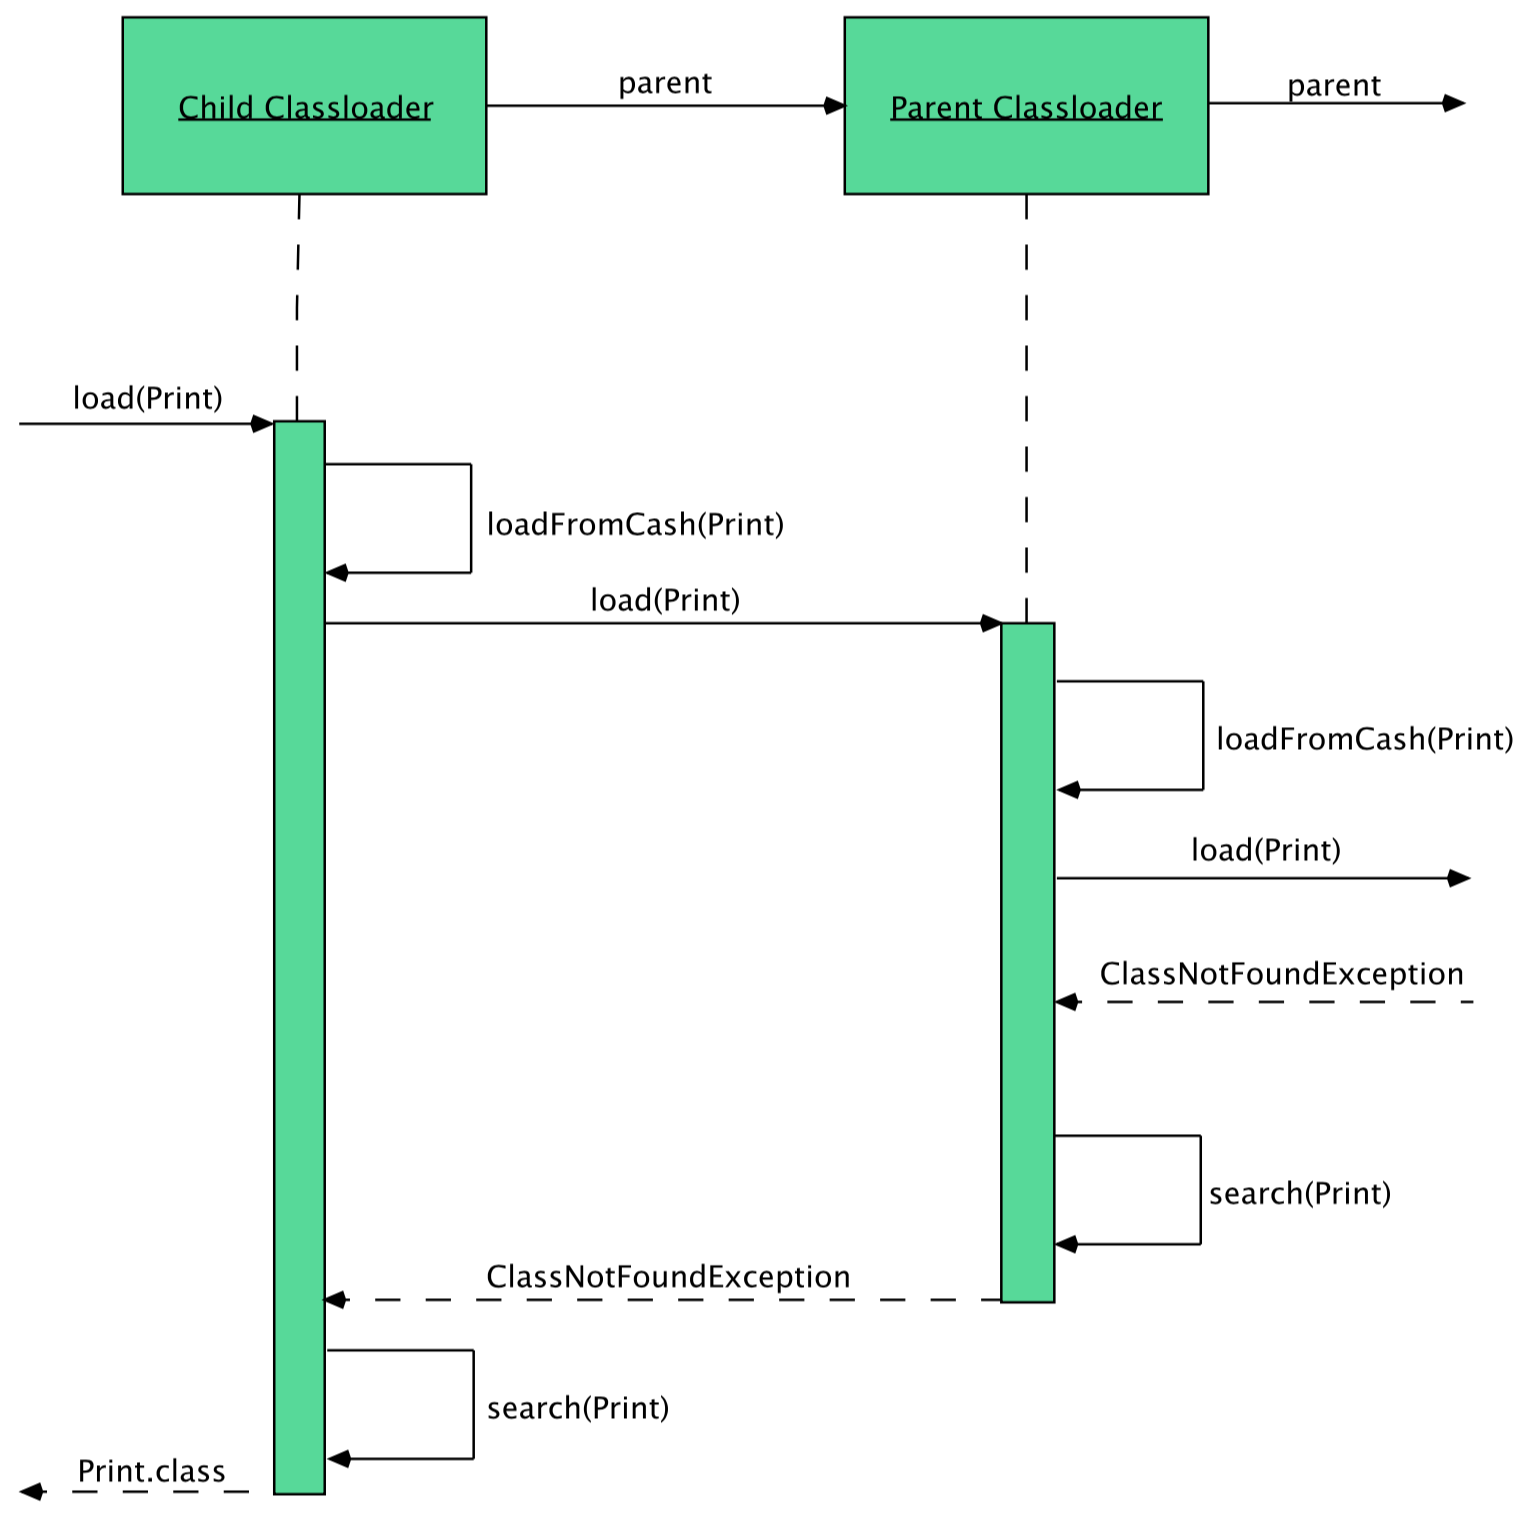
\includegraphics[width=0.9\textwidth]{material/images/deligation.png}
  \caption{Class lookup}
  \label{fig:deligation}
\end{figure}
Wenn während der Suche ein übergeordneter Knoten eine bestimmte Klasse findet, dann wir diese Klasse die Baumhierarchie herunter zu der Anfrage delegiert. Andernfalls versucht der zuständige \textit{Classloader} als letzter die Klasse selbstständig zu laden.
Dies bedeutet, dass eine Klasse normalerweise nicht nur in dem \textit{Classloader} sichtbar ist, der sie geladen hat, sondern auch für alle untergeordneten Instanzen. Dies bedeutet auch, wenn eine Klasse von mehr als einem \textit{Classloader} in einem Baum geladen werden kann, wird immer die Klasse übergeordneten \textit{Classloader} eingelesen. \newline
Dennoch wird vor jedem Laden der Klasse der Cash-Speicher des \textit{Classloaders} nach der gewünschten Instanz durchsucht. Wenn diese existiert, wurde die Suche bereits zuvor durchgeführt und keiner der übergeordneten \textit{Classloader} außer dem jetzigen, war fähig die Anfrage zu beantworten. Somit kann die Suche beschleunigt werden, indem der Type sofort zurückgegeben wird.

\subsubsection{Namensräume}
Geladene Klassen werden sowohl durch den Klassennamen als auch durch den \textit{Classloader} eindeutig identifiziert. Demzufolge werden geladene Klassen in \textit{Namespaces} unterteilt, die vom \textit{Classloader System} individuell behandelt werden.
\newline
Ein \textit{Namespace} ist eine Gruppe von Klassennamen, die von einem bestimmten \textit{Classloader} geladen worden ist. Wenn ein Eintrag für eine Klasse einem \textit{Namespace} hinzugefügt wurde, ist es nicht möglich, eine Klasse mit dem selben Namen und unterschiedlichen Inhalt in den \textit{Namespace} einzubinden. Nichtsdestotrotz können mehrere Kopien einer beliebigen Klasse in die Applikation geladen werden, indem für jede Klasse ein \textit{Classloader} mit dem zusätzlichen \textit{Namespace} erstellt wird. 
\begin{figure}[h]
  \centering
  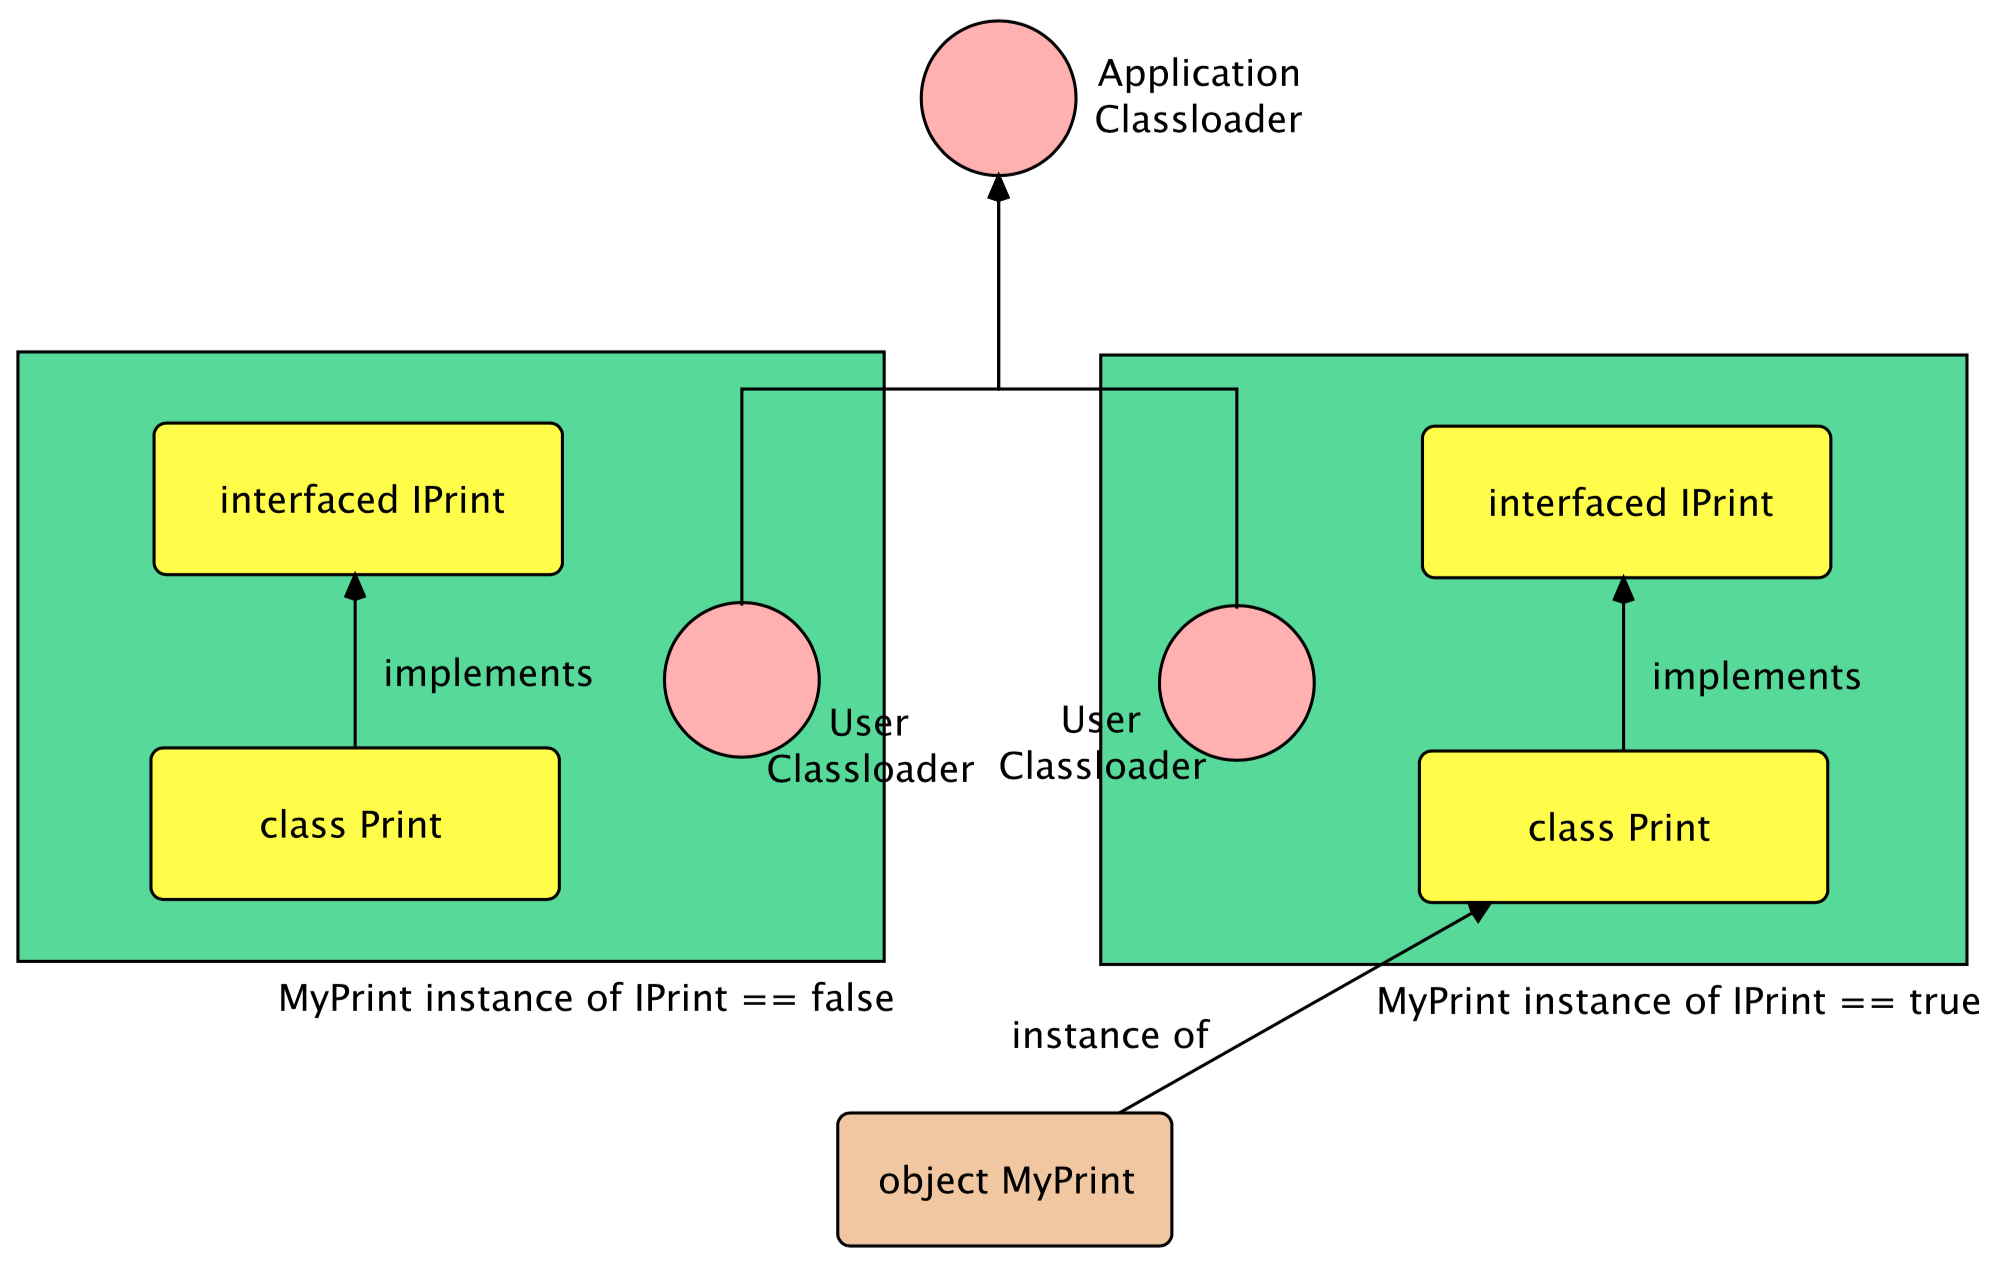
\includegraphics[width=0.9\textwidth]{material/images/namespaces.png}
  \caption{Namensräume}
  \label{fig:namespaces}
\end{figure}
\newline
Abbildung \ref{fig:namespaces} zeigt ein Beispiel für eine Klassenidentitätskrise, die sich ergibt, wenn eine Schnittstelle und die zugehörige Implementierung jeweils von zwei separaten \textit{Classloader} geladen werden. Obwohl die Namen und binären Implementierungen der Schnittstellen und Klassen gleich sind, kann eine Instanz der Klasse von einem \textit{Classloader} nicht als Implementierung des Interfaces von dem anderen \textit{Classloader} erkannt werden. \newline 
Bei Wunsch kann dieser Umstand gelöst werden, indem das Interface eine Ebene höher rutscht und von den Applikation Classloader geladen wird. Somit implementieren beide \textit{Print} Klassen die selbe Schnittstelle.   
\bigbreak
Der Klassen Namensraum bieten zusätzliche Sicherheitsfunktionen wie die Kapselung privat deklarierter Pakete. Die Namensräume verhindern, dass weniger vertrauenswürdiger Code, der aus der Applikation oder benutzerdefinierte \textit{Classloader} geladen worden ist, direkt mit mehr vertrauenswürdigen Klassen interagieren kann. Beispielsweise wird die Kern-API vom \textit{Bootstrap-Classloader} geladen, diese kann \textit{package private} Code enthalten, der bei Anfrage nicht an die unterliegende \textit{Classloader} weitergereicht wird. \newline
Auch wenn ein untergeordneter \textit{Classloader} die Paketstruktur der Core-API nachahmt, wird diese nicht als Teil der Java Core-API anerkannt, da dieser von den falschen Classloader geladen wurde. Somit verhindert die Verwendung von Namensräumen die Möglichkeit spezielle Zugriffsberechtigungen auf private Pakete zu erhalten, indem man selbst geschriebenen Code diesen zuweist.

\subsection{Schnittstelle und Implementierung} % (fold)
\label{sub:Schnittstelle und Implementierung}
Die Schnittstelle(Interface) und Implementierung spielt eine entscheide Rolle für das Nutzen der Klassenfähigkeit.
Eine Schnittstelle ist ein Vertrag, die die Funktionalität alle Klassen, die dieses implementieren beschreibt. 
Wenn eine Klasse eine bestimmte Schnittstelle implementiert, verspricht sie die Umsetzung aller in der Schnittstelle deklarierten Methoden. 
\begin{figure}[h!]
  \centering
  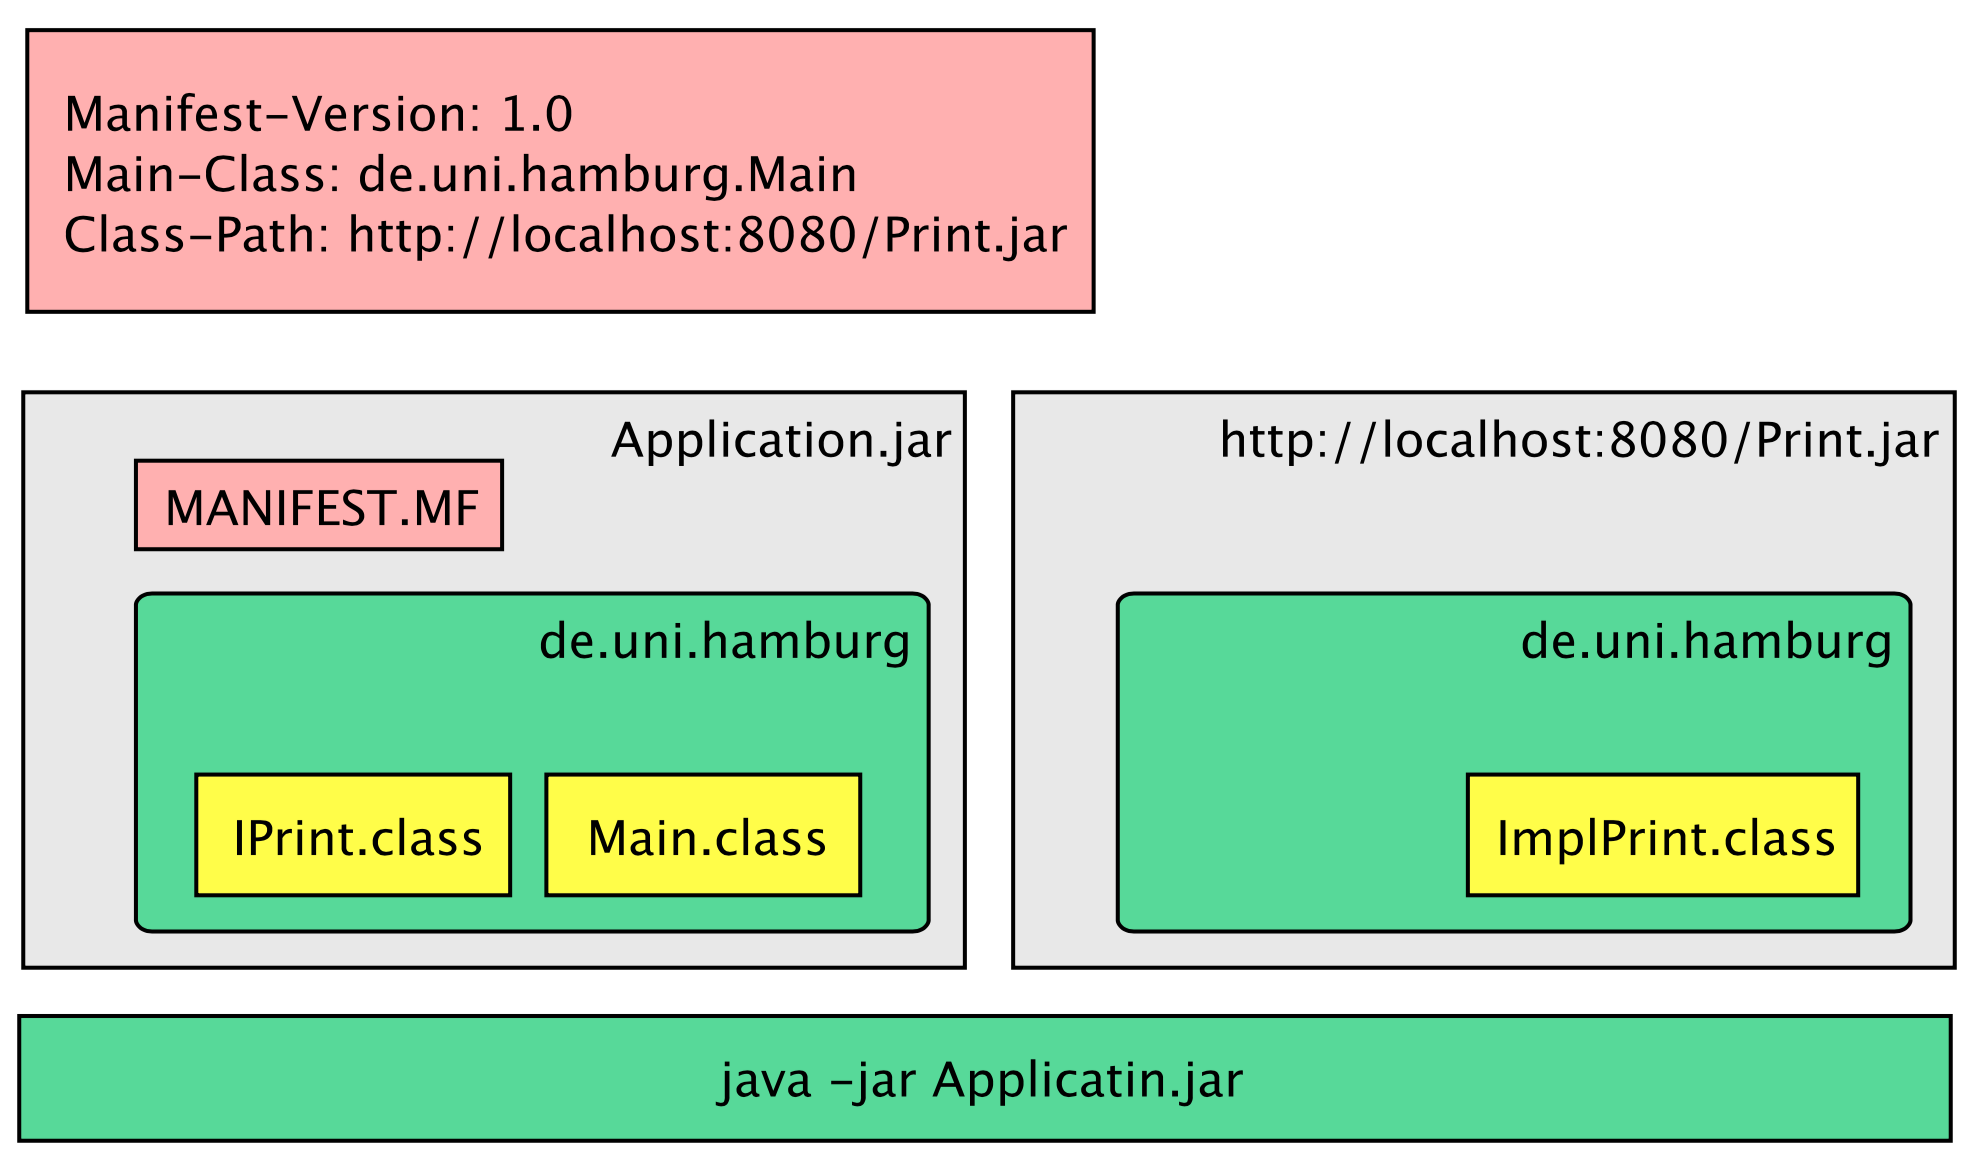
\includegraphics[width=0.8\textwidth]{material/images/Interface.png}
  \caption{Schnittstelle}
  \label{fig:Schnittstelle}
\end{figure}
\newline
Somit wird durch die eigene Umsetzung des Schnittstellenvertrags eine mögliches Verhalten für die Nutzer der Schnittstellenbeschreibung implementiert. 
Daraus folgt ein Kommunikationsvertrag zwischen zwei Objekten, denn wenn eine Klassen eine Schnittstelle implementiert, implementiert diese alle in dieser Schnittstelle deklarierten Methoden und der Methodenaufruf an dieser Klasse wird garantiert ausgeführt. 
\newline
Im Beispiel \ref{fig:Schnittstelle} wird der Vorteil des Schnittstellenvertrags demonstriert, der das Ausführen, für die Applikation unbekannte \textit{PrintImpl} Umsetzung, durch eine einfache Schnittstellenbeschreibung \textit{IPrint} garantiert. Solange die Implementation sich auf der selben Klassenpfadhierarchie befindet wie die Schnittstelle, wird diese während der Laufzeit auf Kompatibilität geprüft und angewandt. Somit kann dynamische Klassenbindungen während der Laufzeit entstehen und Laufzeitbibliotheken ausgetauscht werden ohne die Applikation zu verändern. Hätte man die Schnittstelle nicht genutzt, würde man die Implementation nur als ein Objekt Type instantiieren können und hätte keinen einfachen Zugriff auf ihre Methoden.  


\subsection{Reflaction} 
\label{sec:reflaction}
 % Kurze einleitung 
Reflaction ist die Fähigkeit eines laufenden Programms, sich selbst und seine Softwareumgebung zu analysieren und zu ändern. 
Somit hat die Applikation eine Möglichkeit, durch Reflexion, die Information über ihre Struktur und ihr Verhalten zu erhalten, um wichtige Entscheidungen zu treffen. \newline
Je nachdem welche Information durch die Untersuchung eigener Klassen ausgelesen wurde, können Objekte, die während der Kompilierung nicht präsent waren, mit Hilfe der Reflection-API während der Laufzeit instantiiert, bearbeitet und genutzt werden. Somit ermöglicht Reflection das Arbeiten mit Klassen von den man im Voraus nicht wissen kann, wie zum Beispiel von Klassen, die nach der Applikation entstanden sind.
\bigbreak
 % Überblick: Problemstellung die Reflexion löst 
In vielen Fällen der Applikationsentwicklung möchte man seinen Applikation von andren Nutzern und Entwicklern erweitern lassen, ohne das diese bei jeder Änderungen die komplette Applikation umbauen. 
Somit stellt sich die Frage, wie erstellt man ein Mechanismus der mit beliebigen Klassen arbeiten kann.
Man könnte mit dem zuvor vorgestellten Schnittstellen- und Implementierungsansatz eine gemeinsame Schnittstelle für Erweiterungen definieren, die unserer Applikation mit einer Implementation erweitern lässt und die entsprechenden Methoden definiert. 
Nichtsdestotrotz besteht die Applikation nicht nur aus unserem Code, sondern zusätzlich aus Kern und Drittanbieter Bibliotheken über die wir keine Kontrolle verfügen.
Somit ist die Erweiterung der gesamten Codebasis mit der entsprechenden Schnittstelle oder eine Verschachtelung von \textit{instanceof} Blöcken keine simple oder saubere Lösung. 
Dementsprechend sollte Reflection genutzt werden, diese ermöglicht den Einblick in die Klassenstruktur ohne direkten den Typen zu kennen. Die Klassenstruktur enthalten Informationen über die Klasse selbst, z. B. das Paket und die Superklasse der Klasse sowie die von der Klasse implementierten Schnittstellen. Es enthält auch Details zu den von der Klasse definierten Konstruktoren, Feldern und Methoden.
\bigbreak

%  Sequenzdiagram 

 % Nutzen: Felder Methode, Konstruktoren
Die drei Hauptmerkmale einer Klasse sind ihre Felder, Methoden und Konstruktoren. 
Für die Beschreibung und den Zugriff auf ein Klasse werden diese drei Features in der Reflection-API durch separate Klassen dargestellt: 
\begin{itemize}
\item java.lang.reflect.Field
\item java.lang.reflect.Method
\item java.lang.reflect.Constructor
\end{itemize}
Mit Hilfe der \textit{Class} Objekt eines Typs können die oben genannten Objekte erzeugt und manipuliert werden. Diese bietet eine Schnittstelle für das Abfragen ihrer Struktur an den Nutzer und liefert ein Objekt aus dem \textit{java.lang.reflection} Paket zurück.
\begin{itemize}
\item Field[ ] *.class.getFields();
\item Method[ ] *.class.getDeclaredMethods();
\item Constructor[ ] *.class.getConstructors();
\end{itemize}

\bigbreak
Um den Zusammenhang und den Nutzen von Reflection darzustellen wird in der Abbildung \ref{my-Reflection} ein Szenario durchgespielt, das eine unbekannten Typen mit Hilfe des Konstruktors initialisiert, dessen Methoden aufruft, das Feld bearbeitet und wiedergibt, ohne die Objektstruktur im Voraus zu kennen. 
Des Weiteren ist zu beachten, dass statische Klassenmethoden sowie private Felder und Methoden mit Hilfe von Reflection offen zugänglich gemacht werden können.

\newpage 
 % Bild mit Code der eine Objekt erstellt und Methoden aufrufft. Mit Kommentaren zwischen den Zeilen.
\begin{lstlisting}[caption=Reflection in Aktion,label=my-Reflection,captionpos=b]
    public static void getMethods(@NotNull Class clazz) throws
            NoSuchMethodException, NoSuchFieldException,
            InvocationTargetException, InstantiationException,
            IllegalAccessException {

        Method method;
        Constructor[] ctors = clazz.getDeclaredConstructors();
        Object dynamic = ctors[0].newInstance(4);
        // Methodenaufruf 
        method = clazz.getDeclaredMethod("print");
        method.invoke(dynamic);
        // Methodenaufruf mit Parameter
        method = clazz.getDeclaredMethod("print", String.class, String.class);
        method.invoke(dynamic, "Hello", "World");
        // statischer Aufruf
        method = clazz.getDeclaredMethod("staticPrint");
        method.invoke(null);
        // Aufruf einer privaten Methode
        method = clazz.getDeclaredMethod("doNothing");
        method.setAccessible(true);
        method.invoke(dynamic);
        // Feld Manipulation
        Field field = clazz.getDeclaredField("version");
        field.set(dynamic, 5);
        int version = (int) field.get(dynamic);
        System.out.println(version);
    }
\end{lstlisting}

 % Wo wird Reflection genutzt, wieso ist es so nützlich in der Modernen Software-Entwicklung 
Wie in der Abbildung \ref{my-Reflection} dargestellt ist Reflection ein mächtiges Werkzeug, das aus der morden Softwareentwicklung nicht wegzudenken ist. Refelction wird in jedem Framework verwendet um den Entwickler zu unterstützen. 
\begin{itemize}
  \item Zum Beispiel wird \textit{Dependency Injection} mit Hilfe von Refelction realisiert, indem das Framework (Spring) die entsprechenden Implementierung für ein Interface sucht und initiiert. In Diesem Zusammenhang wird Anhand des \textit{implement} Schlüssels und zusätzlicher Meta-Information aus der Klassen \textit{Annotation} ein eindeutiger Kandidat auserwählt und konstruiert.
\item Beim Sehrealisieren und Deserialisieren von Objekten werden die Objektfelder in JSON und wieder zurück konvertiert, ohne die Feldnamen sowie ihre Anzahl zu kennen.
\item  Der Web-Container wie Tomcat oder WildFly leiteten die Web-Anfragen an das entsprechenden Module durch das Analysieren der \textit{web.xml} und Anfordern der passenden URI.
\item JUnit verwendet Reflection, um die Methoden einer Klasse nach Test-Annotation zu durchsuchen, um diesen anschließend aufzurufen.

 % Sequenz-Diagramm: eines Methodenaufrufs





 % zusammenfassung 
 Java reflection provides access to metadata about fields through metaobjects that are instances of Field. Field objects expose the attributes of a field, such as its name and its modifiers. They also allow access and modification of field values. The convenience facility Array is provided to allow similar functionality for arrays.
Java reflection also allows the ability to access nonpublic members of a class. This ability provides a great deal of benefit to developers seeking to centralize functionality for maintenance purposes. Although encapsulation should normally be preserved, accessibility can be used in a sufficiently general way that does not violate object-oriented principles.
The ability to use metadata about fields gives us concrete benefits. It allows applications like the ones in this chapter to be used on previously developed classes without modification. This ability increases the cohesion of those imple- mentations and broadens their applicability to classes not developed in-house. It also reduces or eliminates the maintenance for applying these implementations to unforeseen future code.

 %% problem wieso keine interfaces oder instanceof genutzt werden und die lösung dazu 

 ✔ Mit Mechanismus für das erweitern der Kernapplikation mit weiteren Code. 
 ✔ dass das System neue Komponenten akzeptieren muss, auch nachdem es erstellt und bereitgestellt wurde.
 ✔ Überleitung von verteilten Code von Interface&Implementierung auf Reflection


Mit der Reflection-API können Sie die Fähigkeiten von Objekten zur Laufzeit ermitteln. Sie wird von der Objektserialisierung verwendet, um Objekte für den Transport über Streams oder für den dauerhaften Speicher zu zerlegen und zu erstellen. Offensichtlich muss die Fähigkeit, Objekte auseinanderzunehmen und ihre inneren Elemente zu sehen, vom Sicherheitsmanager eifrig überwacht werden.


 If George’s team controlled all of the source code, the components could be refactored to implement a common interface that declares setColor. Then, each component could be referenced by that interface type and setColor could be invoked without knowing the concrete type. However, the team does not control the standard Java components or third-party components. Even if they changed the open source components, the open source project might not accept the change, leaving the team with additional maintenance

 Using instanceof and casting to discover concrete types at runtime is another alternative, but it leaves several maintenance problems for George’s team. First, the code would become bloated with conditionals and casts, making it difficult to read and understand. Second, the code would become coupled with each con- crete type. 

 This utility method satisfies the team’s goal of being able to set a component’s color without knowing its concrete type. The method accomplishes its goals with- out invading the source code of any of the components. It also avoids source code bloating, memory bloating, and unnecessary coupling. George has implemented an extremely flexible and effective solution.

 1. Videos gucken
  - Informationen über eine Klasse während der Laufzeit erhalten.
  - Dynamische Datenauslesung.
  - Dynamisches Aktualisieren.
  - Erstelle Type-Instanzen über die wir  keine Informationen während der Laufzeit haben.  
  -



## Input 

Your project manager is committed to a pluggable framework, knowing that the system needs to accept new components even after it is built and deployed. You set up some interfaces and prepare a mechanism for patch- ing your JAR, but you know that this will not completely satisfy the need for pluggability.

Reflection is the ability of a running program to examine itself and its software environment, and to change what it does depending on what it finds.

As we saw in the small example above, the introspection step is followed by behavior change. In general, there are three techniques that a reflection API can use to facilitate behavior change: direct metaobject modification, operations for using metadata (such as dynamic method invocation), and intercession, in which code is permitted to intercede in various phases of program execution.

Applications programmed with reflection adapt more easily to changing requirements. Reflective components are more likely to be reused flawlessly in other applica- tions. These benefits are available in your current Java development kit.


■ security
■ code complexity
■ runtime performance


This line calls the resulting method on obj, passing it the color—This reflective method call can also be referred to as dynamic invocation. Dynamic invoca- tion is a feature that enables a program to call a method on an object at runtime without specifying which method at compile time.

All of this runtime processing also takes more time than casts and static invoca- tion. The method calls for introspection are not necessary if the information is known at compile time. Dynamic invocation introduces latency by resolving which method to call and checking access at runtime rather than at compile time. 

Reflection is a program’s ability to examine and change its behavior and structure at runtime. 

Think of introspection as looking at yourself in a mirror. The mirror provides you with a representation of yourself—your reflection—to examine. Examining yourself in a mirror gives you all sorts of useful information, such as what shirt goes with your brown pants or whether you have something green stuck in your teeth. That information can be invaluable in adjusting the structure of your ward- robe and hygiene. A mirror can also tell you things about your behavior. You can examine whether a smile looks sincere or whether a gesture looks too exaggerated. This information can be critical to understanding how to adjust your behavior to make the right impression on other people.


Similarly, in order to introspect, a program must have access to a representa- tion of itself. This self-representation is the most important structural element of a reflective system. By examining its self-representation, a program can obtain the right information about its structure and behavior to make important decisions.

Metaobjects represent parts of the running application, and, therefore, may describe the base program. Figure 1.1 shows the instanceof relationship between base-level objects and the objects that represent their classes. 

Dynamic invocation enables a program to call a method on an object at runtime without specifying which method at compile time.

 2. Videos hier Zusammenfassen 
 3. Verschmelze Videotext mit Buchtext 
 4. Finde ein Bild wie eine Methode Reflektiv ausgeführt wird, vielleicht in den Videos ? 
 5. Kurzer Satz wo das in Renew auftritt, oder eine starke Andeutung 
 6. Übergang Inversion of Controll 

\section{Inverse of Controll}
\label{sec:inverse_of_controll}

\subsection{Schwächen} % (fold)
\label{sub:schwächen}

\section{Modularisierung}
\label{sec:modularisierung}
- Module gabs schon lagne 
- osg 
- und und und 
- angular 


\section{Einführung}
Ziel des Projekt ist es einen Twitter-Klon zu entwickeln. Als Mikroblogging-Dienst ist die zentrale Funktionalität:
\begin{itemize}
  \item Senden von Tweets
  \item Finden von Tweets (Anzeigen der Tweets in der eigenen Timeline, Suchen nach Schlüsselwörten/Hashtags)
\end{itemize}
Zusätzlich ist selbstverständlich eine Benutzerverwaltung nötig. Ebenso interessant sind Analytics-Funktionalitäten.

In diesem Projekt liegt der Fokus auf der Entwicklung  einer Architektur, die besondere Nicht-Funktionale Anforderungen
erfüllt. Diese ergeben sich aus den Anforderungen an das reale Twitter:
\begin{itemize}
  \item Skalierbarkeit
  \item Erweiterbarkeit um zusätzliche Funktionalität.
\end{itemize}

Geprägt ist Twitter durch enorme Datengeschwindigkeit (Velocity in Gartners Vs). Jede Sekunde werden im
Durchschnitt 6000 Tweets weltweit abgesetzt. Diese Zahlen varieren zudem
stark: Der Rekord liegt bei 140.000 Tweets pro Sekunde\footnote{\url{https://www.brandwatch.com/de/blog/twitter-statistiken/}
\url{http://www.gegen-den-strom.org/twitter/}}.. Zudem werden viele Features von Twitter nach und nach eingeführt,
ohne das Twitter in Wartungspausen geht (gehen musste).

Diesen Herausforderungen sind herkömmliche Webarchitekturen nicht gewachsen. Dieses Projekt entwickelt einen Twitter-Clon
mit den Technologien und einer Architektur, die diesen Anforderen im Prinzip gewachsen ist.

\section{Entwicklung der neuen Architektur}
Ausgangspunkt der Entwicklung der neuen Architektur ist eine einfache Client-Server-Architektur. Es gibt in ihr einen Server
mit viel Rechnenleistung sowie viele Clients. Die Clients verbinden sich mit dem Server, der sie parallel bedient. Die Parallellisierung
erfolgt also auf Thread-/Prozessebene.

Der nächste Schritt ist es, die Datenhaltung in eine Datenbank auszulagern. Es gibt jetzt drei Komponenten: die Clients,
der Webserver und der Datenbankserver. Wenn die Leistung des Serversystems nicht ausreicht gibt es unterschiedliche Möglichkeiten
für mehr Leistung zu sorgen:
\begin{itemize}
  \item Die einzelnen Server mit mehr Leistung auszustatten
  \item Mehr Webserver einzuführen
\end{itemize}
Möglichkeit 1 würde ein Aufrüsten der Server mit schnelleren Prozessoren, mehr Arbeitsspeicher, schnelleren Festplatten etc.
bedeuten. Möglichkeit 2 ist schon etwas komplizierter. Zwar werden die Daten zentral vom Datenbankserver gehalten,
trotzdem können nicht einfach mehr Webserver eingeführt werden. Die Clients müssen noch auf die Webserver verteilt werden.

Diese Aufgabe kann wieder auf zwei Arten erfolgen: Im Netzwerkprotokoll (z.B: über Anycast) oder durch eine zusätzliche
Komponente im Server, nämlich dem Load-Balancer. An ihn kommen alle Anfragen an die Webserver und der Loadbalancer
entscheidet mit mehr oder weniger komplexe Techniken welcher Webserver genutzt werden soll und leitet
den anfragenden Client an diesen Webserver weiter. Dabei achtet diese Komponete z.B. darauf, dass bereits stark
ausgelastete Webserver keine neuen Clients mehr zugewiesen bekommen, sondern nur Webserver mit aktuell
niedriger Auslastung.

Die Parallelisierung erfolgt in dieser Architektur bereits auf vielen Ebenen: Im Loadbalancer, in den Webservern und in der
Datenbank. Die Datenbank führt dafür ausgefeilte Mechansimen zur Verwaltung der parallelen Anfragen und zur
Datenkonsistenz aus.

Diese Architektur wird häufig mit dem LAMP Softwarestack implementiert: Linux als Betriebssystem der Server,
Apache als Webserver, MySQL als Datenbank und PHP als Serverprogrammiersprache.

So weit eine erste Einführung in die Verteilung von Webanwendungen mit herkömmlichen Architekturen.
Nun wollen wir die Art der Verteilung analysieren um darzustellen, weshalb eine andere Architektur für noch
mehr Verteilung nötig ist.

\subsection{Analyse der Verteilung}
Es kommen zwei Techniken der Verteilung zu Einsatz
\begin{itemize}
  \item Erhöhung der Rechenleistung der einzelnen Komponenten
  \item Loadbalancing
\end{itemize}

Die erste Technik wird auch Scale-Up genannt. Durch potentere Hardware kann ein Leistungszuwachs erzielt werden.
Allerdings - und das ist ein zentrales Problem, dass unsere neue Architektur lösen wird - sind dieser Möglichkeit
vergleichsweise enge Grenzen gesetzt. Der Prozessorgeschwindigkeit sind durch die Eigenschaften des verwendeten
Silizium und der Wärmeentwicklung enge Grenzen gesetzt. Über 5 GHz gehen die Taktraten nicht mehr hinaus.
Damit ist bereits bei einem Faktor von ca. 2,5 der Geschwindigkeitserhöhung hier ein Ende gesetzt. Von 2 GHz
geht es bis maximal 5 GHz hoch (und selbst 5 GHz erreichen die wenigsten Prozessoren). Ein Leistungszuwachs
kann jetzt nur noch durch mehr Prozessorkerne und mehr Prozessoren erreicht werden. Durch mehrere Sockel
in den Server (leicht bis zu 4 Stück) und mehr Kernen in den Prozessoren (leicht bis zu 20 Stück) lässt sich hier
bei sehr guter Parallelisierbarkeit der Anwendung\footnote{Amdahl‘s Law zeigt, dass sich durch mehr
Hardware die Geschwindigkeit nicht linear erhöht} theoretisch eine Erhöhung um das 80-fache erreichen.

Hier ist nun die Grenze für das Scale-Up erreicht. Herkömmliche Server lassen sich nun kaum mehr beschleunigen.
Sobald also eine Komponente in unserer Architektur mehr Leistung benötigt weil mehr Client-Anfragen kommen,
als sie bearbeiten kann, müssen wir etwas in der Architektur ändern. Die Ausnahme sind hier die Webserver.
In unserer Architektur können wir bereits mehr Webserver hinzufügen und die Last auf mehr Rechner verteilen,
anstatt auf schnellere Rechner. Das ist ein Grundgedanke unserer neuen Architektur. Im Gegensatz zum Scale-Up
wird dieser Ansatz Scale-Out genannt.

Die Komponente, die dementsprechend als erstes in unserer Architektur geändert werden muss, ist die Datenbank.
Damit beschäftigen wir uns im nächsten Abschnitt.

\subsection{Die Verteilung der Datenbank}
Wir müssen also unsere Datenbank beschleunigen. Wir nehmen an, dass wir kein Scale-Up mehr durchführen können oder
wollen.

Eine Möglichkeit wäre noch die Nutzung von sehr spezialisierter Datenbankhardware. Diese hat sehr große Investitionskosten
und legt einen auf eine spezielle Datenbanksoftware fest. Wir möchten diese deshalb nicht betrachten.

Ein erster Ansatz wäre es, das Load-Balancing der Webserver zu wiederholen. Mehr Datenbankserver und eine Komponente,
die die Anfragen an einen Datenbankserver mit genug verfügbarer Kapazität weiterleitet. Allerdings geht das
nicht mehr so einfach wie bei den Webservern. Die Webserver waren untereinander unabhängig. Die Datenbank ist
das nicht. Man kann nicht einfach einen Datenbankserver nehmen und dort Daten ändern. Wird der Nutzer nun
bei seiner nächsten Anfrage an einen anderen Datenbankserver geleitet, sind die Änderungen dort nicht vorgenommen.
Das ist also keine Alternative.

Aber diesen Ansatz kann man noch verfeinern und schlussendlich gewinnbringend einsetzen.  Das Problem war,
dass die geänderten Daten nur auf einem Server verändert wurden und der User plötzlich auf einen anderen
Datenbankserver landete. Dann muss der Nutzer also immer auf dem gleichen Datenbankserver landen.
Eine einfache Möglichkeit der Verteilung wäre es also, die Nutzer fest auf die Datenbankserver zu verteilen.
Beispielsweise werden alle Nutzer mit Nachnamen, die mit A-K beginnen auf den ersten Datenbankserver zugewiesen,
die anderen auf den zweiten Datenbankserver. In Verwaltungseinrichtungen wird so etwas sogar physisch betrieben.
Wenn der Nutzer nun ein zweites Mal kommt, wird er wieder an den gleichen Datenbankserver weitergeleitet und
seine Daten sind dort aktuell. Diese Aufteilung muss dann aber in der Applikationslogik fest eingebaut werden.
Besser wäre es, wenn das automatisch passieren würde.

Der andere Ansatz wäre es nicht den Benutzer immer auf den gleichen Datenbankserver weiterzuleiten, sondern
die Datenbankserver alle aktuell zu halten. Dann wäre es wieder egal, welchen Datenbankserver er beim nächsten
Besuch nutzt. Allerdings sieht man sofort, dass dann sehr viel Netzwerkverkehr nötig wäre um die Daten auf allen
Server aktuell zu halten. Es ist also zweifelhaft, ob das so viel schneller wäre.

Das wiederum hängt vom Nutzungsprofil ab. Wenn Daten z.B. nur selten geändert werden, aber häufig gelesen,
dann ergibt das wieder Sinn. Der Overhead für das Aktuellhalten der Daten wäre dann sehr gering und
der Leseoperationen würden skalieren. 

\subsection{Ein erste Blick auf die neue Architektur}
Im vorigen Abschnitt haben wir gesehen, dass es nötig wird die Datenbank verteilt auszulegen. Die eine Möglichkeit war
die händische Aufteilung der Anfragen auf verschiedene, unabhängige Datenbankserver. Diese Möglichkeit ist aufwendig.
Eine andere Möglichkeit war das Spiegeln auf mehrere Datenbankserver. Das funktioniert nur dann, wenn die Leseoperationen
die Schreiboperationen weit übertreffen und die Schreiboperationen nur eine Last erzeugen, die ein einzelner Datenbankserver
bearbeiten kann.

Nun betrachten wir eine dritte Möglichkeit: die Verwendung verteilter Datenbanken. Damit werden Datenbankprogramme
bezeichnet, die für den Einsatz auf mehreren Servern gebaut wurden. Sie sind eine Spielart der so genannten NoSQL-Datenbanken.
Zur Skalierung verwenden sie den Scale-Out-Ansatz statt des Scale-Up-Ansatzes. D.h. sie sind so designed, dass man mehr
Leistungsfähigkeit durch das Einbinden weiterer Server erreichen kann. Diese Server bestehen aus herkömmlicher Serverhardware.
Es ist keine spezialisierte Hardware erforderlich. Die Koordinierung erfolgt über Netzwerkprotokolle. Damit wandert die
Skalierbarkeit in die Software. Die Realisierung wird weiter unten in einem gesonderten Kapitel beschrieben.

In der herkömmlichen Architektur wird nun die SQL-Datenbank durch eine verteilte Datenbank ersetzt. Jetzt lässt sich
die benötigte Leistung durch die Verteilung der Datenbank auf genügend Server erreichen. Diese Komponente ist
zusätzlich noch skalierbar, d.h. wenn mehr Leistung benötigt wird, können weitere Server hinzugefügt werden.

Das ist ein Prinzip unserer neuen Architektur: Nicht skalierbare Softwarekomponenten werden durch skalierbare
Softwarekomponenten ausgetauscht. Wir haben mit der Datenbank begonnen. Jetzt ist es Zeit die benötigten Komponenten
für unseren Twitter-Klon zu ermitteln. Im nächsten Schritt setzen wir für die Komponenten Software ein, die skalierbar ist.

\subsection{Benötigte Komponenten}
Unser Twitter-Klon soll die folgende Funktionalität haben:
\begin{itemize}
  \item Nutzerverwaltung: Benutzerkonto mit Login-Funktionalitöt
  \item Kernfunktionalität: Tweets senden und lesen
  \item Tweets entdecken: Tweets suchen und Empfehlungen bekommen
  \item Statistische Auswertungen der Tweets
\end{itemize}

Es gibt offensichtlich eine Frontend-Komponente. Das Backend besteht nun aus verschiedenen Komponenten. Eine Komponente
für die Nutzerverwaltung und eine Komponente für die Kernfunktionalität. Sie greifen auf die Daten in der verteilten Datenbank
zu. Da ein eindeutiger Schlüssel bekannt ist, unterscheidet sich der Zugriff nur in Details vom der Nutzung einer normalen
SQL-Datenbank. Die verteilte Datenbank ist in der Lage die Datenmengen zu handeln und die benötigten Information zurückzuliefern.

Wir verwenden als verteilte Datenbank Cassandra.

Das ist anders beim Suchen der Tweets: Wir gehen davon aus, dass sich enorme Mengen von Tweets in der Datenbank befinden.
Ein naives Durchsuchen wäre sehr teuer und wird deshalb nicht von der verteilten Datenbank angeboten. Wir brauchen also
eine Komponente für das Durchsuchen der Tweets.  Für sie definiert man Kriterien, nach denen gesucht werden kann,
dann liest sie alle Tweets ein und erstellt die entsprechenden verteilten Indexstrukturen. Ab dann ist die Komponente einsatzbereit
und kann dann ebenfalls verteilt unter Zuhilfenahme der vorher erstellten Indexstrukturen die Suchanfragen beantworten.
Zudem hat sie Methoden des Rankings aus dem Dokument Retrieval implementiert um die Suchergebnisse gewerten zurückzugeben.

Die nächste Funktionalität, nämlich die statistische Auswertung der Tweets benötigt wiederum eine eigene Komponente, die
wiederum verteilt arbeiten muss. Für die statistischen Auswertungen werden in Regelfall alle Tweets untersucht,
damit handelt es sich wieder um enorme Datenmengen. Diese können nicht auf einen einzelnen Server geladen werden
und dort ausgewertet werden. Zumindest nehmen wir das bei der Entwicklung der Architektur an. Diese Komponente muss
also verteilte Auswertung unterstützen. Wie das funktioniert, wird ebenso später beschrieben.

Die Komponenten für die Suche existieren bereits und auch die Komponente für die verteilte Auswertung existiert schon:
ElasticSearch für die Suche und Empfehlung und Spark für die verteilte Auswertung.

WIr fassen nochmal zusammen:
\begin{itemize}
  \item Kernfunktionalität: Tweets rein wie raus
  \item Suche und Empfehlung: On-Demand-Berechnung von Antworten auf Suchanfragen unter Nutzung vorbereiter Datenstrukturen
  \item Analytics: Vorberechnung der Analyseergebnisse und dann einfache Rückgabe dieser Ergebnisse auf Anfrage
  \item Realtime-Analytics: Analyse von Stromdaten.
\end{itemize}

Es reicht nicht aus, skalierbare, verteilte Komponenten zu benutzen. Zwischen den Komponenten werden enorme
Datenmengen ausgetauscht. Damit hier keine Flaschenhälse entstehen, müssen auch die Verbindungen zwischen
den Komponenten verteilt sein, wenn sie die ganzen Daten auf einmal verarbeiten. Alternativ müssen die
Komponenten die Daten durchgehend während ihre Entstehung laden.

Es lohnt sich den Datenfluss in unserer Twitter-Klon-Architektur sich genauer anzuschauen.

\subsection{Datenfluss: Stromdatenverarbeitung}
Um zu verdeutlichen, wie der Datenfluss aussieht, betrachten wir kurz unterschiedliche Webanwendungen mit hohem
Leistungsanforderungen
\begin{itemize}
  \item Nachrichtenportal: Hier stehen viele Artikel zum Lesen bereit. Die Anzahl Lesezugriffe (Abrufe von Artikeln)
  übersteigt die Anzahl Schreibzugriffe (Einstellen von neuen Artikeln) deutlich. Es geht also im Wesentlichen darum,
  immer wieder neue Artikel sehr häufig auszuliefern.
  \item Video-On-Demand: Ähnlich wie das Nachrichtportal, nur dass die auszulieferenden Einheiten viel größer
  sind (Videos vs. Texte). Dafür müssen nicht so viele Einheiten in kurzer Zeit ausgeliefert werden
  Auch hier steht die Auslieferung im Vordergrund.
\end{itemize}
Das Anforderungsprofil eines Mikroblogging-Dienst ist etwas anders. Zum einen sind die einzelnen Einheiten sehr klein
(Tweets), zum anderen werden diese von den Nutzern selbst generiert. Und zwar sehr viele in sehr kurzer Zeit.
Die Tweets besonders populäre Nutzer müssen ebenfalls millionfach ausgeliefert werden. Der Fokus liegt aber
längst nicht mehr auf der Auslieferung von Daten. Vielmehr geht es um einen ständigen Strom von Daten
in das System ebenso wie aus dem System heraus. Es geht also um Stromdatenverabeitung.

Dieses Anforderungsprofil harmoniert mit dem Parallelisierungskonzept unser Architektur. Die einzelnen Komponenten
sind verteilt ausgelegt und verteilen die Arbeit auf mehrere einzelne Server. Das geht nun recht einfach. Die
einzelnen Tweets können als (nahezu) unabhängig voneinander betrachtet werden. Sie können insbesondere unabhängig
voneinander gespeichert werden. Damit können die Tweets zur Speicherung an einen beliebigen Datenbankserver weitergeleitet
werden.

Es gibt Ausnahmen von der Unabhängigkeit. Bei einer Folge von Tweets kann es sich um ein Gespräch handeln, d.h. Tweets
antworten aufeinander. Es ist wünschenswert, dass solche Folgen auch vollständig angezeigt werden (können) und nicht
plötzlich ein Tweet im Gespräch fehlt. Über die Realisierung solcher Anforderungen findet sich unten mehr.

Neben der Skalierbarkeit hat unsere Architektur auch weitere Ziele. Es stellt sich noch die Frage, wie die einzelnen
Komponenten verbunden werden und was sie funktional machen.

\subsection{Microservice-Architektur}
Eine ständige Herausforderung bei der Entwicklung von großen System ist die Aufteilung in kleinere Einheiten, die
dann besser gehandelt werden können. Schließlich werden diese Systeme meist von vielen Entwicklern geschrieben,
die häufig auch noch an verschiedenen Standorten sitzen. In unserem Fall werden sogar einige unterschiedliche Technologien
im Backend genutzt.

Der Ansatz der Aufteilung ist es, einzelne Komponenten mit jeweils einer Aufgabe zu entwickeln. Diese Komponenten sollen
unabhänig voneinander entwickelt werden können. Offensichtlich hängen die einzelnen Komponenten in unserem
Twitter-Clon stark voneinander ab. Alle brauchen zum Beispiel Zugriff auf die Tweets. Das ist kein Widerspruch zum 
Microservice-Ansatz, es müssen nur die Schnittstellen vorher erstellt werden (und später eingehalten werden).

Dabei ist es wichtig, dass die Schnittstellen nicht eine spezielle Technologie (insbesondere eine spezielle) Programmiersprache
voraussetzen. In unserer Architektur ist das Austauschformat an den Schnittstellen meist JSON. Die Tweets sind z.B.
JSON-Dateien bei ihrer Erzeugung. Das andere Austauschformat sind die Datenbanktabellen. Für die Datenbank existieren
Connectoren in diversen Programmiersprachen. Die einzelnen Spalten sind zum einen universale Datentypen (Ints, Strings, \dots)
zum anderen Verschachtelungen von den universalen Datentypen.

Hier soll nicht verschwiegen werden, dass dieses Konzept der definierten Schnittstellen vor allem ein Ideal darstellt.
Von ihm wird (und muss) manchmal davon abgewichen werden. Beispielsweise zeigt sich später, dass für die eine
Komponente zusätzliche Felder im JSON notwendig sind. Es ist nicht möglich, dass von Anfang alles
vollständig zu wissen. Zudem sind die Komponenten unabhängig voneinander.
Und nicht alle Komponenten stehen in der Kontrolle der Entwicklungsteams. Werden Daten von außen verwenden,
in unserem Fall benutzen wird Daten von Twitter, so können die das Format festlegen und auch ohne Nachfrage ändern.
In diesem Projekt ist das auch mehrmals passiert. Zwar lässt sich das häufig mit Wrappern, Schema Matching oder auch durch Anpassung
an die Änderungen von außen lösen. Allerdings darf der Aufwand dafür nicht unterschätzt werden.

Der zweite Punkt, der hier kritisch angemerkt werden soll, ist das diese Architektur auch nicht vor den typischen
Data Cleaning-Aufgaben schützt. Eine Definition des Austauschformats bedeutet nicht, dass  a. alle Felder Werte haben,
b. das die Werte korrekt sind und c. dass das Format eingehalten wird. Bei den Twitterdaten heißt das z.B. das bei
weitem nicht alle Tweets Geodaten haben. Trotzdem sind dafür einige Felder vorgesehen. Auch dieses Problem lässt sich
meist lösen. Es zeigte sich aber, dass in unserem Fall einer der Connectoren zur verteilten Datenbank grobe Schwierigkeiten
mit Null-Werten hatte.

Die Microservice-Architektur wird bei uns mit weiteren Konzepten erweitert, wodurch ihr Nutzen nochmal deutlicher
wird. Ohne diese Erweiterungen ist die Mikroservicearchitektur vor allem eine Empfehlung an die Systemdesigner Komponenten möglichst unabhängig
voneinader zu designen und dadurch eine niedrige Kopplung zu erreichen. Das bedeutet auch, programmiersprachenunabhängige Schnittstellen zu bevorzugen.

Wir erweitern das Microservice-Konzept um eine Publish-Subscribe-Architektur und später durch ein Denken in Ereignissen.
Das führt zu einer guten Erweiterbarkeit.

\subsection{Die Publish-Subscribe-Architektur}
Zur Übertragung der Datenströme zwischen den Komponenten nutzen wir Kafka. Es handelt sich dabei um eine verteilte
Streaming Plattform.  Diese Software kümmert sich um die Umsetzung der Datenströme. Sie ist selbst wieder natürlich
skalierbar, und zwar scale-out skalierbar. Im Kern geht es um die Weiterleitung von Nachrichten an alle interessierten Komponenten.
Ein Datenstrom besteht also aus einer Folge von Nachrichten.

Im Kern von Kafka steht das Publish-Subscribe-Modell. Es werden Kanäle angelegt, so genannte Topics. Eine Komponente
kann sich nun bei Kafka für diesen Kanal anmelden ("subscribe") und bekommt ab dann alle Nachrichten von Kafka zugestellt.
Eine Komponente kann dann auch Nachrichten an den Kanal schicken ("publish") und Kafka kümmert sich dann um die Verteilung
an alle Subscriber.

Dies ist eine der Stellen, bei der leicht ein Flaschenhals entstehen kann. Die verteilte Datenbank kann sich nicht direkt
mit Kafka verbinden. Stattdessen muss eine Komponente dazwischen geschaltet werden. Diese Komponente
muss wiederrum verteilt arbeiten. Ansonsten werden alle Tweets über einen Server geleitet. Bis zu einer gewissen
Geschwindigkeit (Tweets pro Zeiteinheit) mag das gut gehen, aber unsere Architektur soll ja gerade so designed sein,
dass man in diesem Fall einfach weitere Server hinzufügen kann.

Ein weiterer Fall sind die Webserver. Wenn sie für den Nutzer Tweets aus der Datenbank anfordern, dann läuft das wieder
über ein solches Topic in Kafka. Das Problem entsteht dann, wenn sich einfach alle Webserver auf das Topic subscriben.
Denn dann erhalten alle Webserver alle Tweets, die von Webservern angefordert worden. Sie sollen aber nur die
Tweets bekommen, die sie auch selbst angefordert haben. Kafka löst das Problem mit so genannten Consumer Groups.
Wie das genau funktioniert, wird weiter unten beschrieben.

Nun wollen wir uns noch anschauen, wie unsere Architektur Erweiterbarkeit unterstützt.

\subsection{Erweiterbarkeit des Systems}
Wir schauen uns das am Beispiel der Realtime-Analytics an. Ihre Aufgabe ist es einfache statistische Auswertungen zu den 
akutell abgesendeten Tweets zu liefern, z.B. die Top 10 Hashtags der aktuellen Stunde. Es gibt jetzt verschiedene Möglichkeiten
an die dafür benötigten Tweets zu kommen:
\begin{itemize}
  \item die Tweets aus der Datenbank lesen
  \item die Tweets vom Webserver nicht nur in die Datenbank schreiben lassen, sondern auch an die Realtime-Analytics-Komponente
zu schicken
\end{itemize}
Beide Verfahren haben erhebliche Nachteile. Das erste Verfahren würde in sehr vielen Datenbankanfragen münden, wenn man
die Stastistiken z.B. jede Sekunde aktualisieren möchte. Das zweite Verfahren würde eine Änderung des Webservers benötigen.

Beide Verfahren sind also nicht geeignet genug. Unsere Architektur kann das Problem hier komfortabel lösen. Es ist ähnlich dem
zweiten Verfahren. Allerdings sendet nicht der Webserver die Daten an die Realtime-Analytics-Komponente. Stattdessen
subscribt sie sich die Realtime-Analytics-Komponente auf das Topic, auf dem der Webserver die Tweets an die Datenbank
sendet. Und schon kümmert sich Kafka darum, dass die Tweets auch dieser Komponente in Echtzeit zur Verfügung gestellt werden.
Es müssen weder Änderungen am Webserver vorgenommen werden, noch an der Datenbank.

Ebenso einfach könnte man die Realtime-Analytics-Komponente auch wieder entfernen. Man meldet sie einfach von Kafka ab.

Hier sieht man, dass eine kleine Änderung im Verständnis der Komponenten vorteilhaft ist: Statt ein Topic für eine Aufgabe
zu benutzen, benutzt man eine Topic für Ereignis in der Realwelt.

\subsection{Denken in Ereignissen}
Bleiben wir im Beispiel des Hinzufügens der Realtime-Analytics-Komponente. Möglicherweise hätte man das Topic, in dem
der Webserver seine Tweets an die Datenbank schickt auch so benannt und gedacht: WebserverTweetsToDatabase. Sobald
jetzt aber die Realtime-Analytics-Komponente hinzugefügt werden soll, passt der Name nicht mehr. Eine Erweiterung auf
WebserverTweetsToDatabaseAndRealtimeAnalytics löst das Problem nicht. Sobald man die nächste Komponente hinzufügen
will, muss man wieder das Topic ändern. Also ziehen wir es zusammen zu WebserverTweetsToX. 

Unsere Architektur schlägt vor nicht in den verbundenen Komponenten zu denken, sondern in Realweltereignissen.
Was wäre nämlich dann, wenn Tweets nicht nur über Webserver gesendet werden könnten, sondern auch über Bots?
Dann würde man schnell bei XTweetsToY als Beschreibung landen. Und das zugehörige Ereignis in der Realwelt wäre:
Der Nutzer sendet einen Tweet ab. Und so sollte nach dieser Regel in der Architektur das Topic auch UserIssuesTweet genannt
werden.


\subsection{Ausfallsicherheit}

Zusätzlich zur Skalierbarkeit der Verteilung können die Komponenten eine gewisse Ausfalltoleranz sicherstellen.
Dadurch dass die Daten auf unterschiedliche Server verteilt werden, können die Daten auch jeweils an mehr als
einen Server geschickt werden.  Bei einer Datenbank können die Daten dann auf mehreren Servern gespeichert werden.
Dadurch entstehen lokale Kopien der Daten. Diese Kopien können dann beim Ausfall die Rolle des ausgefallen
Server übernehmen. Auch die verteilte Auswertesoftware hat ein Mechanismus zur Ausfallsicherheit.

Dabei handelt es sich um einen Tradeoff. Zum einen beim Speicherplatz. Je häufiger die Daten
gespeichert werden, desto mehr Platz wird für die gleiche Menge Daten benötigt. Zum anderen in zeitlicher Hinsicht.
Die Daten werden über das Netzwerk an die Server gesendet. Wenn man nun sicher gehen möchte, dass die Kopien
auch vorhanden sind, muss darauf warten dass die Server Erfolg signalisieren. Dies kann bei mehr als einem Server deutlich
länger dauern als bei einem Server.

Diese Überlegung führt zu Grenzen der Architektur. Durch die Verbindung über das Netzwerk können nicht alle gewünschten
Eigenschaften sichergestellt werden.

\subsection{Grenzen der Architektur}
Normalerweise wird die Software aus unserer Architektur in IP-basierten Netzwerken verwendet werden. Dies sind
so genannte asynchrone Netzwerke. Das heißt, dass die Nachrichtenlaufzeit zwischen zwei Servern ist nicht durch
einen festen Wert begrenzt. Das bedeutet, dass man nicht feststellen kann, ob einen Server ("Knoten") ausgefallen ist
oder die Nachricht nur verzögert ist und noch zugestellt werden würde. In der Praxis wird diese Eigenschaft simuliert,
indem nach einem gewissen Timeout angenommen wird, dass der andere Knoten ausgefallen ist. Er wird dann aus
dem System genommen.

Zum anderen kommt es zu Problemen, wenn die Rechner untereinander nicht mehr erreichbar sind. Dadurch, dass die
Ausführung verteilt wird, sind auch mehrere Server zum Funktionieren erfordert. Dadurch steigt die Ausfallwahrscheinlichkeit
mit der Anzahl der Rechner. Deshalb sind auch Mechanismen zur Ausfallsicherheit notwendig. Trotzdem besteht die
Möglichkeit, dass das Netzwerk zwischen den Servern ausfällt. Das CAP-Theorem besagt, dass in diesem Fall nur
entweder das System an jedem Knoten erreichbar bleibt oder konsistent ist. Für was man sich entscheidet, hängt von den
gewünschten Zieleigenschaften der Architektur ab.
